\subsection[Gettare le fondamenta dell'apprendimento]{Gettare le fondamenta dell'apprendimento}
\begin{frame}
	\frametitle{Data prep: gettare le fondamenta dell'apprendimento}
	
%	\begin{block}{}
		Prima di passare a visionare i \textbf{modelli di apprendimento automatico più diffusi} con i relativi algoritmi, come si può anche osservare in figura, bisogna soffermarci sulle operazioni necessarie a monte del processo di apprendimento: \textbf{la preparazione e il preprocessing dei dati}.
		\newlinedouble
		Quando si costruisce una nuova casa, ci sono cose più importanti da fare prima di pensare alla bellezza dell'architettura o ai particolari estetici.\\
		Prima di tutto ciò vanno \textbf{realizzare delle solide fondamenta} su cui poi innalzare i muri.\\
		Se non si preparano bene le fondamenta – ossia i dati – l'algoritmo non reggerà a lungo quando verrà testato in situazioni in cui si presentano dati reali.
		\begin{figure}[!htbp]
			\centering
			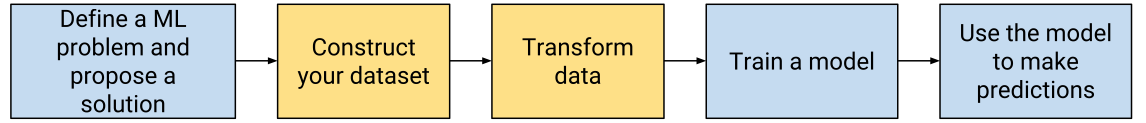
\includegraphics[width=0.9\linewidth]{images/data_prep/build_the_foundation/5phases.png}
					%\caption{Stripe Radar for Fraud Detection}
		\end{figure}

		
%	\end{block}

\end{frame}


%% Per raccogliere e ripulire --> aggiungere il feature enginering
% e il quality of good features


\begin{frame}
	
	\frametitle{Data prep}
	
%	\begin{block}{}
	La \textbf{preparazione e il preprocessing dei dati} consiste in diversi passaggi:
	\begin{enumerate}
		\item ottenere il ground truth, ossia i dati che qualcuno ha correttamente misurato o etichettato
		\item acquisire dati sufficienti da dare in pasto all'algoritmo di apprendimento. Non è possibile sapere a priori quanti sono i dati di cui avrete bisogno, perché tutto dipende dall'algoritmo utilizzato: solo dopo il test riuscirete a capire se le vostre stime soffrono di un eccesso di bias o di varianza dell'algoritmo che avete deciso di adottare
		\item sistemare i dati che avete raccolto in una matrice
		\item gestire i dati problematici, come i casi mancanti (un problema frequente), le distribuzioni distorte, le ridondanze e gli esempi anomali
		\item creare nuove feature (quando occorrono) che risultino particolarmente adatte a fare in modo che l'algoritmo impari come mappare la risposta
	\end{enumerate}
			
%	\end{block}

\end{frame}


\begin{frame}
	
	\frametitle{Data prep}
	
%	\begin{block}{}
		%Tra le operazioni più importanti che spesso è opportuno adottate nella fase di \textbf{preparazione dei dati} ci sono le seguenti:
		Dividiamo quindi i vari task coinvolti nella \textbf{preparazione dei dati} nei seguenti macrogruppi:\\
		\begin{itemize}
			\item {\color{GradientDescentDiagramBlue}raccogliere e ripulire i dati}
			\item {\color{GradientDescentDiagramGreen}sistemare i dati mancanti}
			\item {\color{GradientDescentDiagramOrange}trasformare le distribuzioni}
			\item {\color{GradientDescentDiagramRed}creare proprie features}
			\item etc...
		\end{itemize}		
%	\end{block}

\end{frame}